% !TEX TS-program = pdflatex
% !TEX encoding = UTF-8 Unicode

% This is a simple template for a LaTeX document using the "article" class.
% See "book", "report", "letter" for other types of document.

\documentclass[11pt]{article} % use larger type; default would be 10pt

\usepackage[utf8]{inputenc} % set input encoding (not needed with XeLaTeX)

%%% Examples of Article customizations
% These packages are optional, depending whether you want the features they provide.
% See the LaTeX Companion or other references for full information.

%%% PAGE DIMENSIONS
\usepackage{geometry} % to change the page dimensions
\geometry{a4paper} % or letterpaper (US) or a5paper or....
% \geometry{margin=2in} % for example, change the margins to 2 inches all round
% \geometry{landscape} % set up the page for landscape
%   read geometry.pdf for detailed page layout information
\def\changemargin#1#2{\list{}{\rightmargin#2\leftmargin#1}\item[]}
\let\endchangemargin=\endlist

\usepackage{graphicx} % support the \includegraphics command and options

% \usepackage[parfill]{parskip} % Activate to begin paragraphs with an empty line rather than an indent

%%% PACKAGES
\usepackage{booktabs} % for much better looking tables
\usepackage{array} % for better arrays (eg matrices) in maths
\usepackage{paralist} % very flexible & customisable lists (eg. enumerate/itemize, etc.)
\usepackage{verbatim} % adds environment for commenting out blocks of text & for better verbatim
\usepackage{subfig} % make it possible to include more than one captioned figure/table in a single float
% These packages are all incorporated in the memoir class to one degree or another...

%%% HEADERS & FOOTERS
\usepackage{fancyhdr} % This should be set AFTER setting up the page geometry
\pagestyle{fancy} % options: empty , plain , fancy
\renewcommand{\headrulewidth}{0pt} % customise the layout...
\lhead{}\chead{}\rhead{}
\lfoot{}\cfoot{\thepage}\rfoot{}

%%%
\renewcommand{\_}{\rule{0.2cm}{.5pt}}

%%% SECTION TITLE APPEARANCE
\usepackage{sectsty}
\allsectionsfont{\sffamily\mdseries\upshape} % (See the fntguide.pdf for font help)
% (This matches ConTeXt defaults)

%%% Math theorem styles
\newtheorem{theorem}{Theorem}
\newtheorem{lemma}{Lemma}
\newtheorem{definition}{Definition}

%%%

%%% ToC (table of contents) APPEARANCE
\usepackage[nottoc,notlof,notlot]{tocbibind} % Put the bibliography in the ToC
\usepackage[titles,subfigure]{tocloft} % Alter the style of the Table of Contents
\renewcommand{\cftsecfont}{\rmfamily\mdseries\upshape}
\renewcommand{\cftsecpagefont}{\rmfamily\mdseries\upshape} % No bold!

%%% For Math
\usepackage{amsmath}
\usepackage{amsfonts}
\usepackage{amsbsy}
\usepackage{amssymb}


\makeatletter
\renewcommand*\env@matrix[1][*\c@MaxMatrixCols c]{%
  \hskip -\arraycolsep
  \let\@ifnextchar\new@ifnextchar
  \array{#1}}
\makeatother



%%% For graphics
\usepackage[all]{xy}
\usepackage{tikz}
\usepackage{pgfbaselayers}

\pgfdeclarelayer{background}
\pgfdeclarelayer{foreground}
\pgfsetlayers{background,main,foreground}

%%% END Article customizations

%%% The "real" document content comes below...

\title{Brief Article}
\author{The Author}
\date{13. Januar 2020} % Activate to display a given date or no date (if empty),
         % otherwise the current date is printed 

\begin{document}
\maketitle

\section{Einleitung}

\begin{changemargin}{0pt}{0pt}
Sowie wir für einen Körper $\mathbb{K}$ und eine beliebige Indexmenge $J$ den Vektorraum
\begin{equation}
\mathbb{K}^{J} = \{v: J \longrightarrow \mathbb{K} \}
\end{equation}
der Abbildungen von $J$ nach $\mathbb{K}$ definieren, können wir uns einen Vektor auch vorstellen als
eine Box wo ein Strahl von abgeht, und diesen Strahl können wir mit einem beliebigen Label $i \in J$ versehen, dann
kommt eine Zahl $v_{i} \in \mathbb{K}$ heraus.\\
Zum Beispiel für $J = \{1,\dots,n\}$ sind das $n$-Tupel und den Vektor $v = (7,5,3) \in \mathbb{R}^{\{1,\dots,n\}} =: \mathbb{R}^n$
können wir labeln mit $i = 1$, $i = 2$ oder $i = 3$:
\end{changemargin}
\begin{changemargin}{20pt}{20pt}

\begin{center}
\begin{minipage}{.2\textwidth}

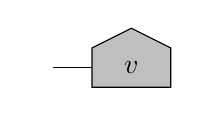
\begin{tikzpicture}
\begin{pgfonlayer}{foreground}
\draw[fill=lightgray] (0-0.5cm,0-0.25cm) -- (0+0.5cm,0-0.25cm) -- (0+0.5cm,0+0.25cm) -- (0,0+0.5cm) -- (0-0.5cm,0+0.25cm) -- cycle;
\node at (0,0) {$v$};
\end{pgfonlayer}
\begin{pgfonlayer}{background}
\draw[-] (0,0) -- (180:1cm);
\node at (180:1.2cm) { };
\end{pgfonlayer}
\end{tikzpicture}

\end{minipage}
%
\begin{minipage}{.2\textwidth}

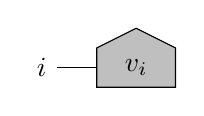
\begin{tikzpicture}
\begin{pgfonlayer}{foreground}
\draw[fill=lightgray] (0-0.5cm,0-0.25cm) -- (0+0.5cm,0-0.25cm) -- (0+0.5cm,0+0.25cm) -- (0,0+0.5cm) -- (0-0.5cm,0+0.25cm) -- cycle;
\node at (0,0) {$v_{i}$};
\end{pgfonlayer}
\begin{pgfonlayer}{background}
\draw[-] (0,0) -- (180:1cm);
\node at (180:1.2cm) {$i$};
\end{pgfonlayer}
\end{tikzpicture}

\end{minipage}
%
\begin{minipage}{.2\textwidth}
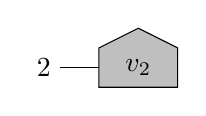
\begin{tikzpicture}
\begin{pgfonlayer}{foreground}
\draw[fill=lightgray] (0-0.5cm,0-0.25cm) -- (0+0.5cm,0-0.25cm) -- (0+0.5cm,0+0.25cm) -- (0,0+0.5cm) -- (0-0.5cm,0+0.25cm) -- cycle;
\node at (0,0) {$v_{2}$};
\end{pgfonlayer}
\begin{pgfonlayer}{background}
\draw[-] (0,0) -- (180:1cm);
\node at (180:1.2cm) {$2$};
\end{pgfonlayer}
\end{tikzpicture}

\end{minipage}
%
\begin{minipage}{.2\textwidth}
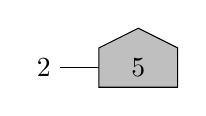
\begin{tikzpicture}
\begin{pgfonlayer}{foreground}
\draw[fill=lightgray] (0-0.5cm,0-0.25cm) -- (0+0.5cm,0-0.25cm) -- (0+0.5cm,0+0.25cm) -- (0,0+0.5cm) -- (0-0.5cm,0+0.25cm) -- cycle;
\node at (0,0) {$5$};
\end{pgfonlayer}
\begin{pgfonlayer}{background}
\draw[-] (0,0) -- (180:1cm);
\node at (180:1.2cm) {$2$};
\end{pgfonlayer}
\end{tikzpicture}

\end{minipage}

\end{center}

\end{changemargin}
%
\begin{changemargin}{0pt}{0pt}
Gegeben zwei Indexmengen $I$ und $J$ können wir uns die $\mathbb{K}$-linearen Abbildungen von $\mathbb{K}^{I}$ nach $\mathbb{K}^{J}$ vorstellen
als Elemente des Vektorraums $\mathbb{K}^{I \times J} := \{m : I \times J \longrightarrow \mathbb{K}\}$. Für $I = \{1,\dots,m\}$ und $J = \{1,\dots,n\}$
schreiben wir wieder verkürzt $\mathbb{K}^{m \times n}$ statt $\mathbb{K}^{\{1,\dots,m\} \times \{1,\dots,n\}}$.
Eine Matrix $m_{ij}$ in dieser Menge können wir darstellen als eine Box, von der zwei Strahlen ausgehen:
\end{changemargin}

\begin{center}
\begin{changemargin}{20pt}{20pt}
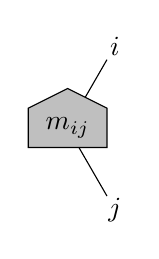
\begin{tikzpicture}
\begin{pgfonlayer}{foreground}
\draw[fill=lightgray] (-0.5cm,-0.25cm) -- (0.5cm,-0.25cm) -- (0.5cm,0.25cm) -- (0,0.5cm) -- (-0.5cm,0.25cm) -- cycle;
\node at (0,0) {$m_{ij}$};
\end{pgfonlayer}
\begin{pgfonlayer}{background}
\draw[-] (0,0) -- (60:1cm);
\node at (60:1.2cm) {$i$};
\draw[-] (0,0) -- (5*60:1cm);
\node at (5*60:1.2cm) {$j$};
\end{pgfonlayer}
\end{tikzpicture}
\end{changemargin}
\end{center}

$
(m_{i,j})_{1 \leq i \leq 4, 1 \leq j \leq 3} =
\begin{pmatrix}[ccc]
  1 & 0 & 2 \\
  0 & 1 & 4 \\
  3 & -2 & -2 \\
  5 & -1 & 6
\end{pmatrix} =
\begin{pmatrix}[c]
  m_{1,\_} \\
  m_{2,\_} \\
  3m_{1,\_} -2m_{2,\_} \\
  5m_{1,\_} -m_{2,\_}
\end{pmatrix}\\
=
\begin{pmatrix}[c]
  1 \\
  0 \\
  3 \\
  5
\end{pmatrix} \otimes m_{1,\_} +
\begin{pmatrix}[c]
  0 \\
  1 \\
  -2 \\
  -1
\end{pmatrix} \otimes m_{2,\_} =
\begin{pmatrix}[c]
  1 \\
  0 \\
  3 \\
  5
\end{pmatrix} \otimes
\begin{pmatrix}[ccc]
  1 & 0 & 2 \\
\end{pmatrix} +
\begin{pmatrix}[c]
  0 \\
  1 \\
  -2 \\
  -1
\end{pmatrix} \otimes
\begin{pmatrix}[ccc]
  0 & 1 & 4
\end{pmatrix} \\
=
(\begin{pmatrix}[c]
  1 \\
  0 \\
  0 \\
  0
\end{pmatrix} +
\begin{pmatrix}[c]
  0 \\
  0 \\
  3 \\
  0
\end{pmatrix} +
\begin{pmatrix}[c]
  0 \\
  0 \\
  0 \\
  5
\end{pmatrix}) \otimes
(\begin{pmatrix}[ccc]
  1 & 0 & 0 \\
\end{pmatrix} +
\begin{pmatrix}[ccc]
  0 & 0 & 2 \\
\end{pmatrix}) \\
+
(\begin{pmatrix}[c]
  0 \\
  1 \\
  0 \\
  0
\end{pmatrix} +
\begin{pmatrix}[c]
  0 \\
  0 \\
  -2 \\
  0
\end{pmatrix} +
\begin{pmatrix}[c]
  0 \\
  0 \\
  0 \\
  -1
\end{pmatrix}) \otimes
(\begin{pmatrix}[ccc]
  0 & 1 & 0
\end{pmatrix} +
\begin{pmatrix}[ccc]
  0 & 0 & 4
\end{pmatrix})\\
=
(1*z_{1}) \otimes (1*s_{1}) + (1*z_{1}) \otimes (2*s_{3})\\
+ (3*z_{3}) \otimes (1*s_{1}) + (3*z_{3}) \otimes (2*s_{3})\\
+ (5*z_{4}) \otimes (1*s_{1}) + (5*z_{4}) \otimes (2*s_{3})\\
+ (1*z_{2}) \otimes (1*s_{2}) + (1*z_{2}) \otimes (4*s_{3})\\
+ (-2*z_{3}) \otimes (1*s_{2}) + (-2*z_{3}) \otimes (4*s_{3})\\
+ (-1*z_{4}) \otimes (1*s_ {2}) + (-1*z_{4}) \otimes (4*s_{3})\\
\\
=
1 z_{1} \otimes s_{1} + 2 z_{1} \otimes s_{3}\\
+ 3 z_{3} \otimes s_{1} + 6 z_{3} \otimes s_{3}\\
+ 5 z_{4} \otimes s_{1} + 10 z_{4} \otimes s_{3}\\
+ 1 z_{2} \otimes s_{2} + 4 z_{2} \otimes s_{3}\\
- 2 z_{3} \otimes s_{2} - 8 z_{3} \otimes s_{3}\\
- z_{4} \otimes s_{2} - 4 z_{4} \otimes s_{3}\\
\\
=
1 z_{1} \otimes s_{1} + 2 z_{1} \otimes s_{3}\\
+ 3 z_{3} \otimes s_{1} - 2 z_{3} \otimes s_{3}\\
+ 5 z_{4} \otimes s_{1} + 6 z_{4} \otimes s_{3}\\
+ 1 z_{2} \otimes s_{2} + 4 z_{2} \otimes s_{3}\\
- 2 z_{3} \otimes s_{2}\\
- z_{4} \otimes s_{2}\\
$
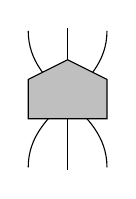
\begin{tikzpicture}

\begin{pgfonlayer}{foreground}

\draw[fill=lightgray] (-0.5cm,-0.25cm) -- (0.5cm,-0.25cm) -- (0.5cm,0.25cm) -- (0,0.5cm) -- (-0.5cm,0.25cm) -- cycle;

\end{pgfonlayer}

\begin{pgfonlayer}{background}
\draw[out=90, in=-90] (4*60:1cm) to (60:1cm);
\draw[-] (90:0.9cm) -- (3*90:0.9cm);
\draw[out=90, in=-90] (5*60:1cm) to (2*60:1cm);
\end{pgfonlayer}

\end{tikzpicture}
\\
\begin{equation}
\begin{pmatrix}[cccc|ccc|c|ccc]
   T_{111} & T_{121} & \dots & T_{1n1} & T_{211} & \dots & T_{2n1} & \dots & T_{m11} & \dots & T_{mn1}  \\
   T_{112} & T_{122} & \dots & T_{1n2} & T_{212} & \dots & T_{2n2} & \dots & T_{m12} & \dots & T_{mn2}  \\
 \vdots & & \ddots & \vdots & \vdots & \ddots & \vdots &  & \vdots & \ddots &  \vdots \\
   T_{11p} & T_{12p} & \dots & T_{1np} & T_{21p} & \dots & T_{2np} & \dots & T_{m1p} & \dots & T_{mnp}
\end{pmatrix}
\end{equation}

Example:

\begin{equation}
T = a_{1} \otimes b_{1} \otimes c_{1} + a_{2} \otimes b_{2} \otimes c_{1}
\end{equation}

has the flattenings

\begin{equation}
T_{C}: 
\begin{pmatrix}[cc|cc]
1 & 0 & 0 & 1 \\
0 & 0 & 0 & 0 \\
\end{pmatrix}
\end{equation}

\begin{equation}
T_{B}: 
\begin{pmatrix}[cc|cc]
1 & 0 & 0 & 0 \\
0 & 0 & 1 & 0 \\
\end{pmatrix}
\end{equation}

\begin{equation}
T_{A}: 
\begin{pmatrix}[cc|cc]
1 & 0 & 0 & 0 \\
0 & 0 & 1 & 0 \\
\end{pmatrix}
\end{equation}
%
%
\begin{changemargin}{20pt}{20pt}

\begin{center}
\begin{minipage}{.2\textwidth}

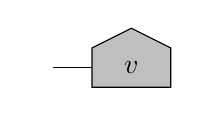
\begin{tikzpicture}
\begin{pgfonlayer}{foreground}
\draw[fill=lightgray] (0-0.5cm,0-0.25cm) -- (0+0.5cm,0-0.25cm) -- (0+0.5cm,0+0.25cm) -- (0,0+0.5cm) -- (0-0.5cm,0+0.25cm) -- cycle;
\node at (0,0) {$v$};
\end{pgfonlayer}
\begin{pgfonlayer}{background}
\draw[-] (0,0) -- (180:1cm);
\node at (180:1.2cm) { };
\end{pgfonlayer}
\end{tikzpicture}

\end{minipage}
%
\begin{minipage}{.2\textwidth}

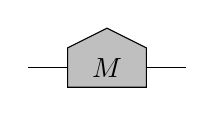
\begin{tikzpicture}
\begin{pgfonlayer}{foreground}
\draw[fill=lightgray] (0-0.5cm,0-0.25cm) -- (0+0.5cm,0-0.25cm) -- (0+0.5cm,0+0.25cm) -- (0,0+0.5cm) -- (0-0.5cm,0+0.25cm) -- cycle;
\node at (0,0) {$M$};
\end{pgfonlayer}
\begin{pgfonlayer}{background}
\draw[-] (0,0) -- (180:1cm);
\draw[-] (0,0) -- (0:1cm);
\end{pgfonlayer}
\end{tikzpicture}

\end{minipage}
%
\begin{minipage}{.2\textwidth}
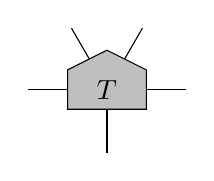
\begin{tikzpicture}
\begin{pgfonlayer}{foreground}
\draw[fill=lightgray] (0-0.5cm,0-0.25cm) -- (0+0.5cm,0-0.25cm) -- (0+0.5cm,0+0.25cm) -- (0,0+0.5cm) -- (0-0.5cm,0+0.25cm) -- cycle;
\node at (0,0) {$T$};
\end{pgfonlayer}
\begin{pgfonlayer}{background}
\draw[-] (0,0) -- (0:1cm);
\draw[-] (0,0) -- (1*60:0.9cm);
\draw[-] (0,0) -- (2*60:0.9cm);
\draw[-] (0,0) -- (180:1cm);
\draw[-] (0,0) -- (270:0.8cm);
\end{pgfonlayer}
\end{tikzpicture}

\end{minipage}
%
\end{center}

\end{changemargin}


\begin{changemargin}{20pt}{20pt}

\begin{center}
\begin{minipage}{.2\textwidth}
%
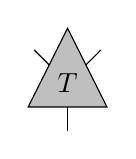
\begin{tikzpicture}
\begin{pgfonlayer}{foreground}
\draw[fill=lightgray] (0-0.5cm,0-0.3cm) -- (0,0+0.7cm) -- (0+0.5cm,0-0.3cm) -- cycle;
\node at (0,0) {$T$};
\end{pgfonlayer}
\begin{pgfonlayer}{background}
\draw[-] (0,0) -- (45:0.6cm);
\draw[-] (0,0) -- (135:0.6cm);
\draw[-] (0,0) -- (270:0.6cm);
\end{pgfonlayer}
\end{tikzpicture}
%
\end{minipage}
\end{center}

\end{changemargin}
%
\begin{changemargin}{20pt}{20pt}

\begin{center}
\begin{minipage}{.2\textwidth}
%
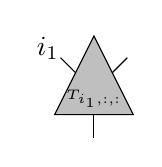
\begin{tikzpicture}
\begin{pgfonlayer}{foreground}
\draw[fill=lightgray] (0-0.5cm,0-0.3cm) -- (0,0+0.7cm) -- (0+0.5cm,0-0.3cm) -- cycle;
\node at (0,0-0.1) {\tiny$T_{i_{1},:,:}$};
\end{pgfonlayer}
\begin{pgfonlayer}{background}
\draw[-] (0,0) -- (45:0.6cm);
\draw[-] (0,0) -- (135:0.6cm);
\node at (137:0.8cm) {$i_{1}$};
\draw[-] (0,0) -- (270:0.6cm);
\end{pgfonlayer}
\end{tikzpicture}
%
\end{minipage}
%
\begin{minipage}{.2\textwidth}
%
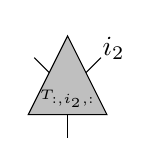
\begin{tikzpicture}
\begin{pgfonlayer}{foreground}
\draw[fill=lightgray] (0-0.5cm,0-0.3cm) -- (0,0+0.7cm) -- (0+0.5cm,0-0.3cm) -- cycle;
\node at (0,0-0.1) {\tiny$T_{:,i_{2},:}$};
\end{pgfonlayer}
\begin{pgfonlayer}{background}
\draw[-] (0,0) -- (45:0.6cm);
\node at (43:0.8cm) {$i_{2}$};
\draw[-] (0,0) -- (135:0.6cm);
\draw[-] (0,0) -- (270:0.6cm);
\end{pgfonlayer}
\end{tikzpicture}
%
\end{minipage}
%
\begin{minipage}{.2\textwidth}
%
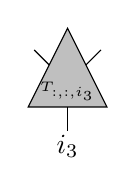
\begin{tikzpicture}
\begin{pgfonlayer}{foreground}
\draw[fill=lightgray] (0-0.5cm,0-0.3cm) -- (0,0+0.7cm) -- (0+0.5cm,0-0.3cm) -- cycle;
\node at (0,0-0.1) {\tiny$T_{:,:,i_{3}}$};
\end{pgfonlayer}
\begin{pgfonlayer}{background}
\draw[-] (0,0) -- (45:0.6cm);
\draw[-] (0,0) -- (135:0.6cm);
\draw[-] (0,0) -- (270:0.6cm);
\node at (270:0.8cm) {$i_{3}$};
\end{pgfonlayer}
\end{tikzpicture}
%
\end{minipage}
\end{center}

\end{changemargin}
%

\begin{changemargin}{20pt}{20pt}

\begin{center}
\begin{minipage}{.2\textwidth}
%
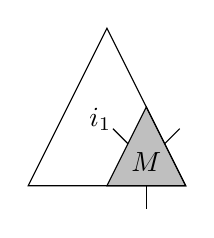
\begin{tikzpicture}
\begin{pgfonlayer}{foreground}
\draw[fill=lightgray] (0-0.5cm,0-0.3cm) -- (0,0+0.7cm) -- (0+0.5cm,0-0.3cm) -- cycle;
\node at (0,0) {$M$};
\draw (0-1.5cm,0-0.3cm) -- (0-0.5,0+1.7cm) -- (0+0.5cm,0-0.3cm) -- cycle;
\end{pgfonlayer}
\begin{pgfonlayer}{background}
\draw[-] (0,0) -- (45:0.6cm);
\draw[-] (0,0) -- (135:0.6cm);
\node at (137:0.8cm) {$i_{1}$};
\draw[-] (0,0) -- (270:0.6cm);
\end{pgfonlayer}
\end{tikzpicture}
%
\end{minipage}
%
\begin{minipage}{.2\textwidth}
%
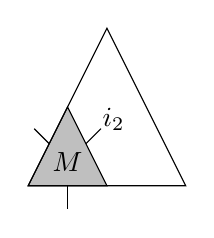
\begin{tikzpicture}
\begin{pgfonlayer}{foreground}
\draw[fill=lightgray] (0-0.5cm,0-0.3cm) -- (0,0+0.7cm) -- (0+0.5cm,0-0.3cm) -- cycle;
\node at (0,0) {$M$};
\draw (0-0.5cm,0-0.3cm) -- (0+1.5cm,0-0.3cm) -- (0+0.5cm,0+1.7cm) -- (0-0.5cm,0-0.3cm) -- cycle;
\end{pgfonlayer}
\begin{pgfonlayer}{background}
\draw[-] (0,0) -- (45:0.6cm);
\node at (43:0.8cm) {$i_{2}$};
\draw[-] (0,0) -- (135:0.6cm);
\draw[-] (0,0) -- (270:0.6cm);
\end{pgfonlayer}
\end{tikzpicture}
%
\end{minipage}
%
\begin{minipage}{.2\textwidth}
%
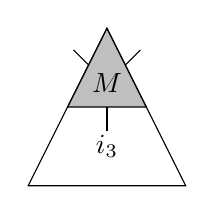
\begin{tikzpicture}
\begin{pgfonlayer}{foreground}
\draw[fill=lightgray] (0-0.5cm,0-0.3cm) -- (0,0+0.7cm) -- (0+0.5cm,0-0.3cm) -- cycle;
\node at (0,0) {$M$};
\draw (0,0+0.7cm) -- (0-1cm,0-1.3cm) -- (0+1cm,0-1.3cm) -- cycle;
\end{pgfonlayer}
\begin{pgfonlayer}{background}
\draw[-] (0,0) -- (45:0.6cm);
\draw[-] (0,0) -- (135:0.6cm);
\draw[-] (0,0) -- (270:0.6cm);
\node at (270:0.8cm) {$i_{3}$};
\end{pgfonlayer}
\end{tikzpicture}
%
\end{minipage}
\end{center}

\end{changemargin}

Das bedeutet umgekehrt, man kann jeden d-Stufigen Tensor T auch auffassen als einen (d+k)-stufigen Tensor S, bei dem k Moden mit festen Labeln\\
$i_{j} \in I_{j}$ für $j = d+1,\dots,k$ versehen sind. Genauso wie man einen Vektor $v \in \mathbb{R}^{n}$ als Spalte $M_{\_,j}$ einer Matrix $M_{i,j} \in \mathbb{R}^{m\times n}$
auffassen kann.


\begin{changemargin}{20pt}{20pt}
\begin{center}
%
\begin{minipage}{.2\textwidth}
% tensor T 5 modes
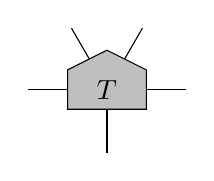
\begin{tikzpicture}
\begin{pgfonlayer}{foreground}
\draw[fill=lightgray] (0-0.5cm,0-0.25cm) -- (0+0.5cm,0-0.25cm) -- (0+0.5cm,0+0.25cm) -- (0,0+0.5cm) -- (0-0.5cm,0+0.25cm) -- cycle;
\node at (0,0) {$T$};
\end{pgfonlayer}
\begin{pgfonlayer}{background}
\draw[-] (0,0) -- (0:1cm);
\draw[-] (0,0) -- (1*60:0.9cm);
\draw[-] (0,0) -- (2*60:0.9cm);
\draw[-] (0,0) -- (180:1cm);
\draw[-] (0,0) -- (270:0.8cm);
\end{pgfonlayer}
\end{tikzpicture}
\end{minipage}
%
\begin{minipage}{.2\textwidth}
% tensor S inside of T
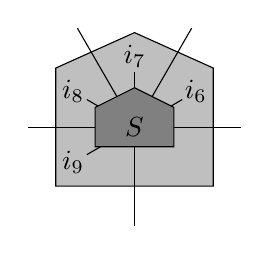
\begin{tikzpicture}
\begin{pgfonlayer}{foreground}
\draw[fill=gray] (0-0.5cm,0-0.25cm) -- (0+0.5cm,0-0.25cm) -- (0+0.5cm,0+0.25cm) -- (0,0+0.5cm) -- (0-0.5cm,0+0.25cm) -- cycle;
\node at (0,0) {$S$};
\end{pgfonlayer}
\draw[-] (0,0) -- (0:1.35cm);
\draw[-] (0,0) -- (1*60:1.45cm);
\draw[-] (0,0) -- (2*60:1.45cm);
\draw[-] (0,0) -- (180:1.35cm);
\draw[-] (0,0) -- (270:1.25cm);
\begin{pgfonlayer}{background}
\draw[fill=lightgray] (0-1cm,0-0.75cm) -- (0+1cm,0-0.75cm) -- (0+1cm,0+0.75cm) -- (0,0+1.2cm) -- (0-1cm,0+0.75cm) -- cycle;
\draw[-] (0,0) -- (1*30:0.7cm);
\node  at (1*30:0.9cm) {$i_{6}$};
\draw[-] (0,0) -- (3*30:0.7cm);
\node  at (3*30:0.9cm) {$i_{7}$};
\draw[-] (0,0) -- (5*30:0.7cm);
\node  at (5*30:0.9cm) {$i_{8}$};
\draw[-] (0,0) -- (7*30:0.7cm);
\node  at (7*30:0.9cm) {$i_{9}$};
\end{pgfonlayer}
\end{tikzpicture}
\end{minipage}
%
\end{center}
\end{changemargin}
$
T
\begin{pmatrix}[c]
i_{1}, i_{2}, i_{3}, i_{4}, i_{5}
\end{pmatrix}
=
S
\begin{pmatrix}[c]
i_{1}, i_{2}, i_{3}, i_{4}, i_{5}, \overline{i_{6}}, \overline{i_{7}}, \overline{i_{8}}, \overline{i_{9}}
\end{pmatrix}$ für feste $\overline{i_{j}} \in I_{j}, j\in\{6,\dots,9\}$.

\subsection{A subsection}

\begin{lemma}
\[ \mathbb{R}^{\pmb{\mathrm{I}}} = \bigotimes_{j=1}^{d} \mathbb{R}^{I_{j}} \]
\end{lemma}

\begin{definition}
\pmb{\emph{Äußerer Produktrang}}
\begin{equation}
\mathrm{rank}_{\otimes}(\mathbf{T}) := \mathrm{min}\left\{
r \in \mathbb{N}_{0} : \exists v_{\nu}^{(j)} \in \mathbb{R}^{I_{j}} \emph{ mit }
\mathbf{T} = \sum_{\nu = 1}^{r} \bigotimes_{j = 1}^{d} v_{\nu}^{(j)}
\right\}
,
\mathbf{T} \in \mathbb{R}^{\mathbf{I}}.
\end{equation}
\end{definition}

%
% tensor T
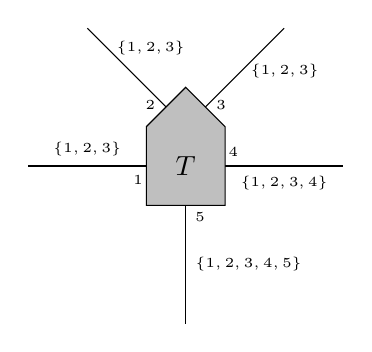
\begin{tikzpicture}
\begin{pgfonlayer}{foreground}
\draw[fill=lightgray] (0-0.5cm,0-0.5cm) -- (0+0.5cm,0-0.5cm) -- (0+0.5cm,0+0.5cm) -- (0,0+1cm) -- (0-0.5cm,0+0.5cm) -- cycle;
\node at (0,0) {$T$};
\end{pgfonlayer}
\begin{pgfonlayer}{background}
\draw[-] (0-0.5cm,0) -- node [below,pos=0.07] {\tiny1} node [above,midway] {\tiny$\{1,2,3\}$} (0-2cm,0); %j=1
\draw[-] (0-0.25cm,0+0.75cm) -- node [below,pos=0.2] {\tiny2} node [right,near end] {\tiny$\{1,2,3\}$} (0-1.25cm,0.5cm+1.25cm); %j=2
\draw[-] (0+0.25cm,0+0.75cm) -- node [below,pos=0.2] {\tiny3} node [right,pos=0.45] {\tiny$\{1,2,3\}$} (0+1.25cm,0.5cm+1.25cm); %j=3
\draw[-] (0+0.5cm,0) -- node [above,pos=0.07] {\tiny4} node [below,midway] {\tiny$\{1,2,3,4\}$} (0+2cm,0); %j=4
\draw[-] (0,0-0.5cm) -- node [right,pos=0.1] {\tiny5} node [right,midway] {\tiny$\{1,2,3,4,5\}$} (0,-0.5cm-1.5cm); %j=5
\end{pgfonlayer}
\end{tikzpicture}
\\

$\mathbf{T} \in \mathbb{R}^{3\times3\times3\times4\times5}$ hat also $3\cdot3\cdot3\cdot4\cdot5 = 540$ Einträge.\\

%
% core tensor X
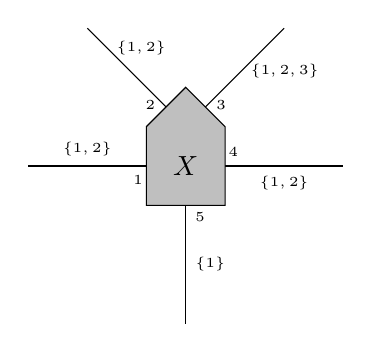
\begin{tikzpicture}
\begin{pgfonlayer}{foreground}
\draw[fill=lightgray] (0-0.5cm,0-0.5cm) -- (0+0.5cm,0-0.5cm) -- (0+0.5cm,0+0.5cm) -- (0,0+1cm) -- (0-0.5cm,0+0.5cm) -- cycle;
\node at (0,0) {$X$};
\end{pgfonlayer}
\begin{pgfonlayer}{background}
\draw[-] (0-0.5cm,0) -- node [below,pos=0.07] {\tiny1} node [above,midway] {\tiny$\{1,2\}$} (0-2cm,0); %j=1
\draw[-] (0-0.25cm,0+0.75cm) -- node [below,pos=0.2] {\tiny2} node [right,near end] {\tiny$\{1,2\}$} (0-1.25cm,0.5cm+1.25cm); %j=2
\draw[-] (0+0.25cm,0+0.75cm) -- node [below,pos=0.2] {\tiny3} node [right,pos=0.45] {\tiny$\{1,2,3\}$} (0+1.25cm,0.5cm+1.25cm); %j=3
\draw[-] (0+0.5cm,0) -- node [above,pos=0.07] {\tiny4} node [below,midway] {\tiny$\{1,2\}$} (0+2cm,0); %j=4
\draw[-] (0,0-0.5cm) -- node [right,pos=0.1] {\tiny5} node [right,midway] {\tiny$\{1\}$} (0,-0.5cm-1.5cm); %j=5
\end{pgfonlayer}
\end{tikzpicture}

% 
% core tensor X with matrices U1,...,U5
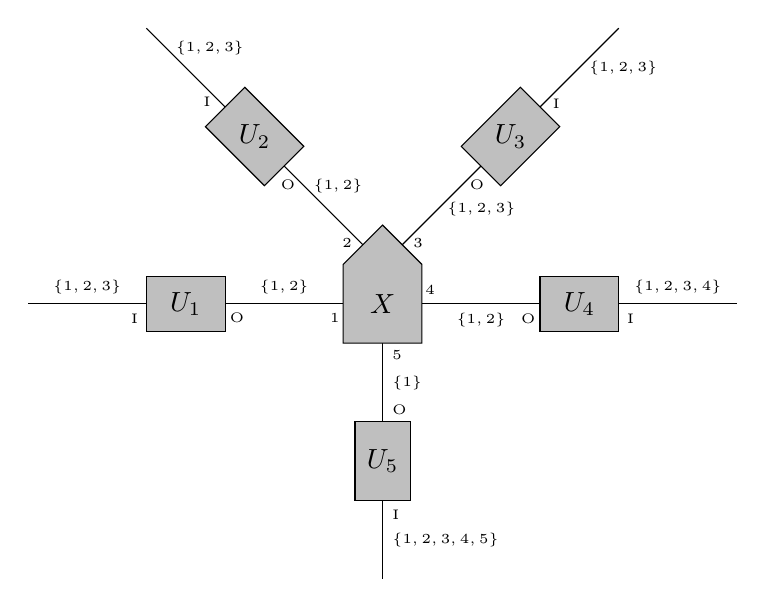
\begin{tikzpicture}
\begin{pgfonlayer}{foreground}
\draw[fill=lightgray] (0-0.5cm,0-0.5cm) -- (0+0.5cm,0-0.5cm) -- (0+0.5cm,0+0.5cm) -- (0,0+1cm) -- (0-0.5cm,0+0.5cm) -- cycle;
\node at (0,0) {$X$};
\end{pgfonlayer}
\begin{pgfonlayer}{background}
\draw[-] (0-0.5cm,0) -- node [below,pos=0.9] {\tiny O} node [below,pos=0.07] {\tiny1} node [above,midway] {\tiny$\{1,2\}$} (0-2cm,0); %j=1
\draw[-] (0-0.25cm,0+0.75cm) -- node [below,pos=0.95] {\tiny O} node [below,pos=0.2] {\tiny2} node [right,near end] {\tiny$\{1,2\}$}
 (0-1.25cm,0.5cm+1.25cm); %j=2
\draw[-] (0+0.25cm,0+0.75cm) -- node [below,pos=0.95] {\tiny O} node [below,pos=0.2] {\tiny3} node [right,pos=0.45] {\tiny$\{1,2,3\}$} 
(0+1.25cm,0.5cm+1.25cm); %j=3
\draw[-] (0+0.5cm,0) -- node [below,pos=0.9] {\tiny O} node [above,pos=0.07] {\tiny4} node [below,midway] {\tiny$\{1,2\}$} 
(0+2cm,0); %j=4
\draw[-] (0,0-0.5cm) -- node [right,pos=0.85] {\tiny O} node [right,pos=0.15] {\tiny5} node [right,midway] {\tiny$\{1\}$} 
(0,-0.5cm-1cm); %j=5
\end{pgfonlayer}
%U1 p=(-2.5cm,0)
\draw[fill=lightgray] (-2.5cm-0.5cm,0-0.35cm) -- (-2.5cm+0.5cm,0-0.35cm) -- (-2.5cm+0.5cm,0+0.35cm) -- (-2.5cm-0.5cm,0+0.35cm) -- cycle;
\node at (-2.5cm,0) {$U_{1}$};
\draw[-] (-2.5cm-0.5cm,0) -- node [below,pos=0.1] {\tiny I} node [above,midway] {\tiny$\{1,2,3\}$} (-2.5cm-2cm,0);
%U2 p=(-1.5cm,2cm)
\draw[fill=lightgray] (-1.5cm,2cm-0.5cm) -- (-1.5cm-0.75cm,2cm-0.5cm+0.75cm) -- (-1.5cm-0.25cm,2cm+0.75cm) -- (-1.5cm+0.5cm,2cm) -- cycle;
\node at (-1.5cm-0.125cm,2cm+0.125cm) {$U_{2}$};
\draw[-] (-2cm,2.5cm) -- node [left,pos=0.06] {\tiny I} node [right,near end] {\tiny$\{1,2,3\}$} (-3cm,3.5cm);
%U3 p=(1.5cm,2cm)
\draw[fill=lightgray] (1.5cm-0.5cm,2cm) -- (1.5cm+0.25cm,2cm+0.75cm) -- (1.5cm+0.75cm,2cm+0.25cm) -- (1.5cm,2cm-0.5cm) -- cycle;
\node at (1.5cm+0.125cm,2cm+0.125cm) {$U_{3}$};
\draw[-] (1.5cm+0.5cm,2cm+0.5cm) -- node [right,pos=0.04] {\tiny I} node [right,midway] {\tiny$\{1,2,3\}$} (3cm,3.5cm);
%U4 p=(2.5cm,0)
\draw[fill=lightgray] (2.5cm-0.5cm,0-0.35cm) -- (2.5cm+0.5cm,0-0.35cm) -- (2.5cm+0.5cm,0+0.35cm) -- (2.5cm-0.5cm,0+0.35cm) -- cycle;
\node at (2.5cm,0) {$U_{4}$};
\draw[-] (2.5cm+0.5cm,0) -- node [below,pos=0.1] {\tiny I} node [above,pos=0.5] {\tiny$\{1,2,3,4\}$} (2.5cm+2cm,0);
%U5 p=(0,-2cm)
\draw[fill=lightgray] (0-0.35cm,-2cm+0.5cm) -- (0-0.35cm,-2cm-0.5cm) -- (0+0.35cm,-2cm-0.5cm) -- (0+0.35cm,-2cm+0.5cm) -- cycle;
\node at (0,-2cm) {$U_{5}$};
\draw[-] (0,-2.5cm) -- node [right,pos=0.18] {\tiny I}  node [right,midway] {\tiny$\{1,2,3,4,5\}$} (0,-3.5cm);
\end{tikzpicture}

$ \mathbf{T} = (U_{1},\dots,U_{5}) \cdot X =\\
\left(
\begin{pmatrix}[cc]
  0 & 2\\
  1 & 4\\
  7 & 9
\end{pmatrix} \otimes
\begin{pmatrix}[cc]
  0 & 1\\
  1 & 3\\
  5 & -9
\end{pmatrix} \otimes
\begin{pmatrix}[ccc]
  1 & 0 & -6\\
  -3 & 1 & 4\\
  7 & 8 & 9
\end{pmatrix} \otimes
\begin{pmatrix}[cccc]
  0 & 2 & 1 & 3\\
  1 & 4 & -2 & 4
\end{pmatrix} \otimes
\begin{pmatrix}[ccccc]
  0 & 2 & 3 & -7 & 8
\end{pmatrix}
\right) \cdot X$

wobei $X \in \mathbb{R}^{2\times 2\times 3\times 2\times 1}$ d.h. es gibt $2\cdot 2\cdot 3\cdot 2\cdot 1 = 24$ Einträge zu speichern,
dazu noch die Einträge in den Matrizen $3\cdot2 + 3\cdot2 + 3\cdot3 + 2\cdot4 +1\cdot5 = 34$ macht insgesamt $24+34=58$ Einträge
statt $540$. Dass man denselben Datengehalt in so viel weniger Platz darstellen kann, macht deutlich, dass unter den 540 möglichen Einträgen
viel leerer Raum war.

%
%kommutierendes Dreiecks-Diagramm
\begin{center}
\begin{minipage}{.33\textwidth}
\end{minipage}
\begin{minipage}{.33\textwidth}
\begin{xy}
%vertices
(10,35)*+{V_{1}\times\dots\times V_{d}}="o1";(35,35)*+{U}="o2";
(18,25)*+{\circlearrowleft};
(10,10)*+{\bigotimes^{d}_{j=1} V_{j}}="u1";
%arrows
{\ar@{->}_{\Phi} "u1";"o2"};%
{\ar@{->}^{\hspace{5mm}\varphi} "o1";"o2"};%
{\ar@{->}_{\otimes} "o1";"u1"};%
\end{xy}
\end{minipage}
\begin{minipage}{.33\textwidth}
\end{minipage}
\end{center}



% 
% core tensor X with matrices U1,...,U5, r = (1,1,1,1,1)
\begin{center}
\begin{minipage}{.33\textwidth}
\end{minipage}
\begin{minipage}{.33\textwidth}
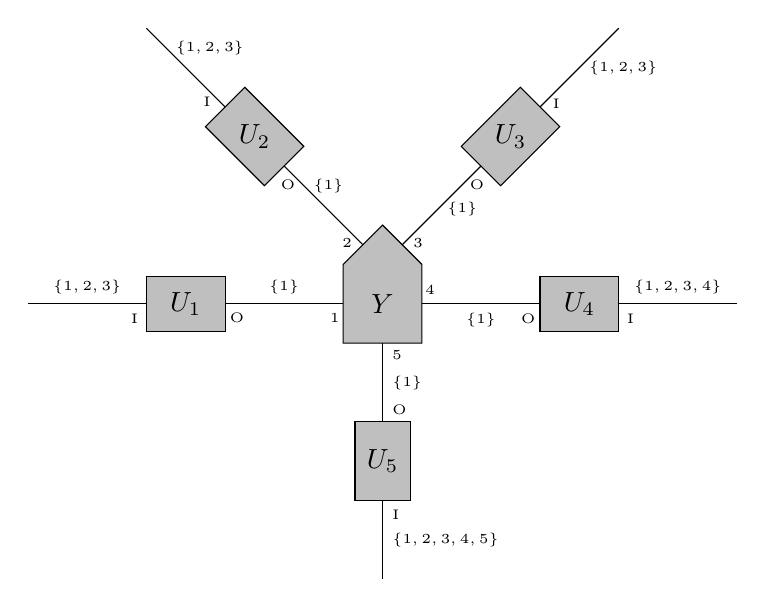
\begin{tikzpicture}
\begin{pgfonlayer}{foreground}
\draw[fill=lightgray] (0-0.5cm,0-0.5cm) -- (0+0.5cm,0-0.5cm) -- (0+0.5cm,0+0.5cm) -- (0,0+1cm) -- (0-0.5cm,0+0.5cm) -- cycle;
\node at (0,0) {$Y$};
\end{pgfonlayer}
\begin{pgfonlayer}{background}
\draw[-] (0-0.5cm,0) -- node [below,pos=0.9] {\tiny O} node [below,pos=0.07] {\tiny1} node [above,midway] {\tiny$\{1\}$} (0-2cm,0); %j=1
\draw[-] (0-0.25cm,0+0.75cm) -- node [below,pos=0.95] {\tiny O} node [below,pos=0.2] {\tiny2} node [right,near end] {\tiny$\{1\}$}
 (0-1.25cm,0.5cm+1.25cm); %j=2
\draw[-] (0+0.25cm,0+0.75cm) -- node [below,pos=0.95] {\tiny O} node [below,pos=0.2] {\tiny3} node [right,pos=0.45] {\tiny$\{1\}$} 
(0+1.25cm,0.5cm+1.25cm); %j=3
\draw[-] (0+0.5cm,0) -- node [below,pos=0.9] {\tiny O} node [above,pos=0.07] {\tiny4} node [below,midway] {\tiny$\{1\}$} 
(0+2cm,0); %j=4
\draw[-] (0,0-0.5cm) -- node [right,pos=0.85] {\tiny O} node [right,pos=0.15] {\tiny5} node [right,midway] {\tiny$\{1\}$} 
(0,-0.5cm-1cm); %j=5
\end{pgfonlayer}
%U1 p=(-2.5cm,0)
\draw[fill=lightgray] (-2.5cm-0.5cm,0-0.35cm) -- (-2.5cm+0.5cm,0-0.35cm) -- (-2.5cm+0.5cm,0+0.35cm) -- (-2.5cm-0.5cm,0+0.35cm) -- cycle;
\node at (-2.5cm,0) {$U_{1}$};
\draw[-] (-2.5cm-0.5cm,0) -- node [below,pos=0.1] {\tiny I} node [above,midway] {\tiny$\{1,2,3\}$} (-2.5cm-2cm,0);
%U2 p=(-1.5cm,2cm)
\draw[fill=lightgray] (-1.5cm,2cm-0.5cm) -- (-1.5cm-0.75cm,2cm-0.5cm+0.75cm) -- (-1.5cm-0.25cm,2cm+0.75cm) -- (-1.5cm+0.5cm,2cm) -- cycle;
\node at (-1.5cm-0.125cm,2cm+0.125cm) {$U_{2}$};
\draw[-] (-2cm,2.5cm) -- node [left,pos=0.06] {\tiny I} node [right,near end] {\tiny$\{1,2,3\}$} (-3cm,3.5cm);
%U3 p=(1.5cm,2cm)
\draw[fill=lightgray] (1.5cm-0.5cm,2cm) -- (1.5cm+0.25cm,2cm+0.75cm) -- (1.5cm+0.75cm,2cm+0.25cm) -- (1.5cm,2cm-0.5cm) -- cycle;
\node at (1.5cm+0.125cm,2cm+0.125cm) {$U_{3}$};
\draw[-] (1.5cm+0.5cm,2cm+0.5cm) -- node [right,pos=0.04] {\tiny I} node [right,midway] {\tiny$\{1,2,3\}$} (3cm,3.5cm);
%U4 p=(2.5cm,0)
\draw[fill=lightgray] (2.5cm-0.5cm,0-0.35cm) -- (2.5cm+0.5cm,0-0.35cm) -- (2.5cm+0.5cm,0+0.35cm) -- (2.5cm-0.5cm,0+0.35cm) -- cycle;
\node at (2.5cm,0) {$U_{4}$};
\draw[-] (2.5cm+0.5cm,0) -- node [below,pos=0.1] {\tiny I} node [above,pos=0.5] {\tiny$\{1,2,3,4\}$} (2.5cm+2cm,0);
%U5 p=(0,-2cm)
\draw[fill=lightgray] (0-0.35cm,-2cm+0.5cm) -- (0-0.35cm,-2cm-0.5cm) -- (0+0.35cm,-2cm-0.5cm) -- (0+0.35cm,-2cm+0.5cm) -- cycle;
\node at (0,-2cm) {$U_{5}$};
\draw[-] (0,-2.5cm) -- node [right,pos=0.18] {\tiny I}  node [right,midway] {\tiny$\{1,2,3,4,5\}$} (0,-3.5cm);
\end{tikzpicture}
\end{minipage}
\begin{minipage}{.33\textwidth}
\end{minipage}
\end{center}

$ \mathbf{T} = (U_{1},\dots,U_{5}) \cdot Y = \left(
\begin{pmatrix}[c]
  1 \\
  0 \\
  3 
\end{pmatrix}^{\top},
\begin{pmatrix}[c]
  1 \\
  1 \\
  3 
\end{pmatrix}^{\top},
\begin{pmatrix}[c]
  0 \\
  1 \\
  7 
\end{pmatrix}^{\top},
\begin{pmatrix}[c]
  1 \\
  1 \\
  3 \\
  -2
\end{pmatrix}^{\top},
\begin{pmatrix}[c]
  2 \\
  7 \\
  6 \\
  0 \\
  8
\end{pmatrix}^{\top} \right) \otimes Y \\
= 
Y_{[1,1,1,1,1]} 
\begin{pmatrix}[c]
  1 \\
  0 \\
  3 
\end{pmatrix} \otimes
\begin{pmatrix}[c]
  1 \\
  1 \\
  3 
\end{pmatrix} \otimes
\begin{pmatrix}[c]
  0 \\
  1 \\
  7 
\end{pmatrix} \otimes
\begin{pmatrix}[c]
  1 \\
  1 \\
  3 \\
  -2
\end{pmatrix} \otimes
\begin{pmatrix}[c]
  2 \\
  7 \\
  6 \\
  0 \\
  8
\end{pmatrix}
$

Um an den Kern-Tensor $\mathbf{Y} = Y_{[1,1,1,1,1]} =: Y$ zu kommen, rechnet man mit den einzelnen Matrizen das 5-stufige Matrix-Vektor-Produkt

$Y = \mathbf{T} \times_{1} 
\begin{pmatrix}[c]
  1 \\
  0 \\
  3 
\end{pmatrix} \times_{2}
\begin{pmatrix}[c]
  1 \\
  1 \\
  3 
\end{pmatrix} \times_{3}
\begin{pmatrix}[c]
  0 \\
  1 \\
  7 
\end{pmatrix} \times_{4}
\begin{pmatrix}[c]
  1 \\
  1 \\
  3 \\
  -2
\end{pmatrix} \times_{5}
\begin{pmatrix}[c]
  2 \\
  7 \\
  6 \\
  0 \\
  8
\end{pmatrix}
$
\end{document}
